\chapter{Multiple and Polynomial Regression}
\label{chap:multiple_poly_regression}

% ========================================
% SECTION 1: INTRODUCTION
% ========================================
\section{Introduction: Beyond a Single Feature}
In Chapter 1, we predicted Package using only CGPA. But in the real world, many factors influence salary: Projects, Internships, Communication Skills, etc.

\begin{definition}
\textbf{Multiple Linear Regression}: A regression model that predicts a target variable using \textbf{two or more} input features.
\end{definition}

\section{Geometric Intuition}
How does the ``Best Fit Line'' change when we add more features?
\begin{itemize}
    \item \textbf{1 Feature}: The model is a \textbf{Line} in 2D space.
    \item \textbf{2 Features}: The model is a \textbf{Plane} in 3D space.
    \item \textbf{3+ Features}: The model is a \textbf{Hyperplane} in N-dimensional space.
\end{itemize}

\begin{figure}[htbp]
\centering
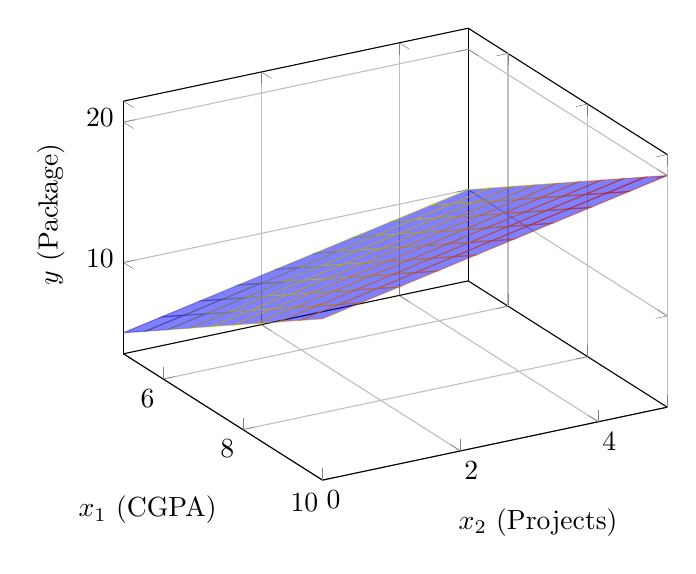
\begin{tikzpicture}
    \begin{axis}[
        view={60}{30},
        xlabel=$x_1$ (CGPA), ylabel=$x_2$ (Projects), zlabel=$y$ (Package),
        width=0.7\textwidth,
        grid=major
    ]
    % Plane: y = 2*x1 + 1*x2 - 5
    \addplot3[surf, opacity=0.5, color=blue, domain=5:10, domain y=0:5, samples=10] {2*x + 1*y - 5};
    \end{axis}
\end{tikzpicture}
\caption{In Multiple Linear Regression with 2 features, the model is a flat plane.}
\label{fig:mlr_plane}
\end{figure}

\section{Mathematical Formulation}
The equation extends naturally:
\begin{equation}
    y = \beta_0 + \beta_1 x_1 + \beta_2 x_2 + \ldots + \beta_p x_p
\end{equation}
\begin{itemize}
    \item $\beta_0$: Intercept (baseline value when all features are zero).
    \item $\beta_1, \beta_2, \ldots, \beta_p$: Coefficients (weights for each feature).
    \item For $p$ features, we have $p+1$ parameters to estimate.
\end{itemize}

% ========================================
% SECTION: MATRIX FORMULATION
% ========================================
\section{Matrix Formulation}
For computational efficiency, we express everything using matrices.

\subsection{Setting Up the Matrices}
\begin{itemize}
    \item $\mathbf{Y}$: Vector of target values (size: $n \times 1$).
    $$\mathbf{Y} = \begin{bmatrix} y_1 \\ y_2 \\ \vdots \\ y_n \end{bmatrix}$$
    
    \item $\mathbf{X}$: Design Matrix (size: $n \times (p+1)$). We prepend a column of 1s to handle the intercept $\beta_0$.
    $$\mathbf{X} = \begin{bmatrix} 
    1 & x_{11} & x_{12} & \cdots & x_{1p} \\
    1 & x_{21} & x_{22} & \cdots & x_{2p} \\
    \vdots & \vdots & \vdots & \ddots & \vdots \\
    1 & x_{n1} & x_{n2} & \cdots & x_{np}
    \end{bmatrix}$$
    
    \item $\boldsymbol{\beta}$: Vector of coefficients (size: $(p+1) \times 1$).
    $$\boldsymbol{\beta} = \begin{bmatrix} \beta_0 \\ \beta_1 \\ \vdots \\ \beta_p \end{bmatrix}$$
\end{itemize}

The predicted values are: $\hat{\mathbf{Y}} = \mathbf{X} \boldsymbol{\beta}$

% ========================================
% SECTION: OLS DERIVATION (DETAILED)
% ========================================
\section{Deriving the Normal Equation (OLS)}
We want to find the $\boldsymbol{\beta}$ that minimizes the Sum of Squared Errors (SSE).

\subsection{Step 1: Define the Error}
The error (residual) vector is:
$$\mathbf{e} = \mathbf{Y} - \hat{\mathbf{Y}} = \mathbf{Y} - \mathbf{X}\boldsymbol{\beta}$$

\subsection{Step 2: Define the Loss Function (SSE)}
The Sum of Squared Errors in matrix form is:
$$E = \mathbf{e}^T \mathbf{e} = (\mathbf{Y} - \mathbf{X}\boldsymbol{\beta})^T (\mathbf{Y} - \mathbf{X}\boldsymbol{\beta})$$

\subsection{Step 3: Expand the Expression}
Using the transpose rule $(AB)^T = B^T A^T$:
$$E = (\mathbf{Y}^T - \boldsymbol{\beta}^T \mathbf{X}^T)(\mathbf{Y} - \mathbf{X}\boldsymbol{\beta})$$

Multiply out (FOIL method):
\begin{align}
E &= \mathbf{Y}^T \mathbf{Y} - \mathbf{Y}^T \mathbf{X}\boldsymbol{\beta} - \boldsymbol{\beta}^T \mathbf{X}^T \mathbf{Y} + \boldsymbol{\beta}^T \mathbf{X}^T \mathbf{X} \boldsymbol{\beta}
\end{align}

\textbf{Key Observation}: The terms $\mathbf{Y}^T \mathbf{X}\boldsymbol{\beta}$ and $\boldsymbol{\beta}^T \mathbf{X}^T \mathbf{Y}$ are both scalars (1$\times$1 matrices). A scalar equals its transpose, so:
$$\mathbf{Y}^T \mathbf{X}\boldsymbol{\beta} = (\boldsymbol{\beta}^T \mathbf{X}^T \mathbf{Y})^T = \boldsymbol{\beta}^T \mathbf{X}^T \mathbf{Y}$$

Therefore, we can combine them:
\begin{equation}
E = \mathbf{Y}^T \mathbf{Y} - 2\boldsymbol{\beta}^T \mathbf{X}^T \mathbf{Y} + \boldsymbol{\beta}^T \mathbf{X}^T \mathbf{X} \boldsymbol{\beta}
\label{eq:sse_expanded}
\end{equation}

\subsection{Step 4: Differentiate with Respect to $\boldsymbol{\beta}$}
To find the minimum, we take the derivative and set it to zero.

\textbf{Matrix Calculus Rules}:
\begin{itemize}
    \item $\frac{\partial}{\partial \mathbf{x}} (\mathbf{a}^T \mathbf{x}) = \mathbf{a}$ (derivative of a linear term)
    \item $\frac{\partial}{\partial \mathbf{x}} (\mathbf{x}^T \mathbf{A} \mathbf{x}) = 2\mathbf{A}\mathbf{x}$ (derivative of a quadratic form, when $\mathbf{A}$ is symmetric)
\end{itemize}

Applying these rules to Equation \ref{eq:sse_expanded}:
\begin{align}
\frac{\partial E}{\partial \boldsymbol{\beta}} &= 0 - 2\mathbf{X}^T \mathbf{Y} + 2\mathbf{X}^T \mathbf{X} \boldsymbol{\beta}
\end{align}

\subsection{Step 5: Set Gradient to Zero and Solve}
Setting the derivative to zero:
$$-2\mathbf{X}^T \mathbf{Y} + 2\mathbf{X}^T \mathbf{X} \boldsymbol{\beta} = 0$$

Rearranging:
$$\mathbf{X}^T \mathbf{X} \boldsymbol{\beta} = \mathbf{X}^T \mathbf{Y}$$

Multiply both sides by $(\mathbf{X}^T \mathbf{X})^{-1}$ (assuming it exists):
$$(\mathbf{X}^T \mathbf{X})^{-1} \mathbf{X}^T \mathbf{X} \boldsymbol{\beta} = (\mathbf{X}^T \mathbf{X})^{-1} \mathbf{X}^T \mathbf{Y}$$

Since $(\mathbf{X}^T \mathbf{X})^{-1} (\mathbf{X}^T \mathbf{X}) = \mathbf{I}$ (Identity matrix):
\begin{equation}
\boxed{\boldsymbol{\beta} = (\mathbf{X}^T \mathbf{X})^{-1} \mathbf{X}^T \mathbf{Y}}
\label{eq:normal_equation_final}
\end{equation}

This is the \textbf{Normal Equation} (OLS Closed-Form Solution).

\subsection{When Does This Fail?}
The solution requires $(\mathbf{X}^T \mathbf{X})^{-1}$ to exist. This fails when:
\begin{enumerate}
    \item \textbf{Multicollinearity}: Two or more features are perfectly correlated (e.g., $x_2 = 2x_1$).
    \item \textbf{More features than samples}: $p > n$.
\end{enumerate}
\textbf{Solution}: Use Regularization (Ridge Regression) or drop correlated features.

\subsection{Computational Complexity}
Computing the inverse of a $(p+1) \times (p+1)$ matrix has time complexity $O(p^3)$.
\begin{itemize}
    \item For small $p$ (10-100 features): OLS is fast.
    \item For large $p$ (100,000+ features): Use Gradient Descent instead.
\end{itemize}

% ========================================
% SECTION: POLYNOMIAL REGRESSION
% ========================================
\section{Polynomial Regression}
What if the relationship is curved, not linear?

\begin{definition}
\textbf{Polynomial Regression}: A technique where we generate new features by raising existing features to powers ($x^2, x^3, \ldots$), and then apply standard Linear Regression.
\end{definition}

\textbf{Key Insight}: The algorithm itself does not change. We only transform the input data.

\textbf{For one feature $x$}:
\begin{itemize}
    \item \textbf{Degree 1}: $y = \beta_0 + \beta_1 x$ (Straight line).
    \item \textbf{Degree 2}: $y = \beta_0 + \beta_1 x + \beta_2 x^2$ (Parabola).
    \item \textbf{Degree 3}: $y = \beta_0 + \beta_1 x + \beta_2 x^2 + \beta_3 x^3$ (Cubic curve).
\end{itemize}

\textbf{Why is it still ``Linear'' Regression?}
The model is \textit{non-linear} in terms of $x$, but it is still \textit{linear} in terms of the coefficients $\beta$. We are doing Multiple Linear Regression with derived features ($x, x^2, x^3$).

\section{Implementation in Python}
\begin{lstlisting}[language=Python, caption=Normal Equation Implementation]
import numpy as np

def fit_normal_equation(X, y):
    """Fit Multiple LR using Normal Equation."""
    # Step 1: Add column of 1s for intercept
    n = X.shape[0]
    X_b = np.c_[np.ones((n, 1)), X]  # Shape: (n, p+1)
    
    # Step 2: Apply Normal Equation
    # beta = (X^T X)^(-1) X^T y
    XtX = X_b.T @ X_b           # (p+1, p+1)
    XtX_inv = np.linalg.inv(XtX) # Inverse
    Xty = X_b.T @ y              # (p+1, 1)
    beta = XtX_inv @ Xty         # (p+1, 1)
    
    return beta

# Example
X = np.array([[1], [2], [3], [4], [5]])  # 1 feature
y = np.array([2, 4, 5, 4, 5])
beta = fit_normal_equation(X, y)
print(f"Intercept: {beta[0]:.2f}, Slope: {beta[1]:.2f}")
\end{lstlisting}

\section{HOTS: Interview Questions}
\textbf{Q1: Is Polynomial Regression a linear or non-linear model?}
\begin{itemize}
    \item It is a \textbf{Linear Model} because it is linear with respect to the \textit{parameters} (coefficients $\beta$). The non-linearity is in the features, not the model itself.
\end{itemize}

\textbf{Q2: Walk me through the Normal Equation derivation.}
\begin{itemize}
    \item We define the error as $\mathbf{e} = \mathbf{Y} - \mathbf{X}\boldsymbol{\beta}$.
    \item We minimize SSE = $\mathbf{e}^T\mathbf{e}$.
    \item Expand, differentiate w.r.t. $\boldsymbol{\beta}$, set to zero.
    \item Solve to get $\boldsymbol{\beta} = (\mathbf{X}^T\mathbf{X})^{-1}\mathbf{X}^T\mathbf{Y}$.
\end{itemize}

\textbf{Q3: Why is feature scaling important in Polynomial Regression?}
\begin{itemize}
    \item If $x = 1000$, then $x^2 = 1,000,000$ and $x^3 = 1,000,000,000$. Feature magnitudes explode, causing numerical instability.
    \item Always use \texttt{StandardScaler} before polynomial transformation.
\end{itemize}
